\beginsong{Es wollt ein Bauer früh aufstehn}[wuw={Volkslied aus dem 15. Jahrhundert, Fassung von Thomas Fritz und Erich Schmeckenbecher, 1978}, bo={142}, pfii={76}, pfiii={57}]

\beginverse
\endverse
\centering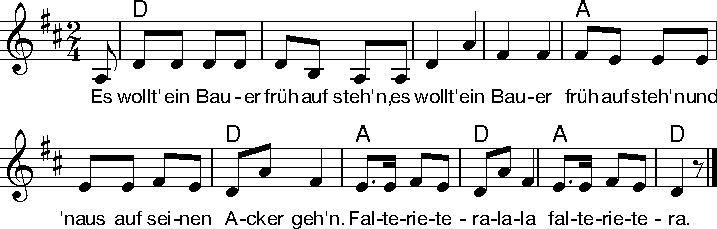
\includegraphics[width=1\textwidth]{Noten/Lied042.pdf}

\beginverse
Und \[D]als der Bauer nach Hause kam, und als der Bauer nach \[A]Hause kam,
da wollt er was zu \[D]fressen ham'.
\endverse

\beginchorus
\[A]Fal-te-rie-te-\[D]ra-la-la, \[A]fal-te-rie-te-\[D]ra.
\endchorus

\beginverse
''Ach ^Lieschen, koch mir Hirsebrei, ach Lieschen, koch mir ^Hirsebrei
mit Bratkartoffeln, ^Spiegelei!''
\endverse

\beginverse
Und ^als der Bauer saß und fraß, und als der Bauer ^saß und fraß,
da rumpelt in der ^Kammer was.
\endverse

\beginverse
''Ach ^liebe Frau, was ist denn das? Ach liebe Frau, was ^ist denn das?
Da rumpelt in der ^Kammer was.''
\endverse

\beginverse
''Ach ^lieber Mann, das ist der Wind, ach lieber Mann, das ^ist der Wind,
der raschelt da im ^Küchenspind.''
\endverse

\beginverse
Der ^Bauer sprach: ''Will selber seh'n'', der Bauer sprach: ''Will ^selber seh'n,
will selber in die ^Kammer geh'n.''
\endverse

\beginverse
Und ^als der Bauer in d' Kammer kam, und als der Bauer in d' ^Kammer kam,
zog der Pfaff' die ^Hosen an.
\endverse

\beginverse
''Ach ^Pfaff', was machst in meinem Haus? Ach Pfaff', was machst in ^meinem Haus?
Ich werf dich gleich zum ^Fenster raus.''
\endverse

\beginverse
Der ^Pfaff', der sprach: ''Was ich verricht' '', der Pfaff, der sprach: ''Was ^ich verricht',
dein' Frau, die kann die ^Beichte nicht.''
\endverse

\beginverse
Da ^nahm der Bauer ein' Ofenscheit, da nahm der Bauer ein' ^Ofenscheit
und schlug den Pfaffen, ^bis er schreit.
\endverse

\beginverse
Der ^Pfaffe schrie: ''O Schreck, o Graus!'', der Pfaffe schrie: ''O ^Schreck, o Graus!''
und hing den Arsch zum ^Fenster raus.
\endverse

\beginverse
Da ^kamen die Leut' von nah und fern, da kamen die Leut' von ^nah und fern
und dachten, es sei der ^Morgenstern.
\endverse

\beginverse
Der ^Morgenstern, der war es nicht, der Morgenstern, der ^war es nicht,
es war des Pfaffen ^Arschgesicht.
\endverse

\beginverse
So ^soll es allen Pfaffen geh'n, so soll es allen ^Pfaffen geh'n,
die nachts zu fremden ^Weibern geh'n.
\endverse

\beginverse
Und ^die Moral von der Geschicht', und die Moral von ^der Geschicht':
Trau' nie des Pfaffen ^Arschgesicht!
\endverse

\endsong

\beginscripture{}
Pfaffe ist ein wenig gebrauchtes Wort für einen Pfarrer beziehungsweise einen Geistlichen.
\endscripture
